\documentclass[11pt, oneside]{report}
\usepackage{geometry}
\usepackage{graphicx}
\usepackage{amssymb}
\usepackage{amsmath}
\usepackage{apacite}
\usepackage[numbers]{natbib}
\usepackage{fancyhdr}
\usepackage{lastpage}
\usepackage{graphicx, wrapfig, subcaption, setspace, booktabs}
\usepackage[toc,page]{appendix}
\usepackage[T1]{fontenc}
\usepackage[font=small, labelfont=bf]{caption}
\usepackage{fourier}
\usepackage[protrusion=true, expansion=true]{microtype}
\usepackage[english]{babel}
\usepackage{sectsty}
\usepackage{url, lipsum}
\usepackage{mathtools}
\usepackage{listings}
\DeclarePairedDelimiter{\floor}{\lfloor}{\rfloor}

\geometry{letterpaper}

\newcommand{\HRule}[1]{\rule{\linewidth}{#1}}
\onehalfspacing
\setcounter{tocdepth}{5}
\setcounter{secnumdepth}{5}

%-------------------------------------------------------------------------------
% HEADER & FOOTER
%-------------------------------------------------------------------------------
\pagestyle{fancy}
\fancyhf{}
\setlength\headheight{15pt}
\fancyhead[L]{Student ID: 3032162875}
\fancyhead[R]{University of California, Berkeley}
\fancyfoot[R]{Page \thepage\ of \pageref{LastPage}}

%-------------------------------------------------------------------------------
% TITLE PAGE
%-------------------------------------------------------------------------------
\title{
  \HRule{0.5pt} \\
  \LARGE \textbf{\uppercase{Forecasting Monthly Active Users for Adobe Creative Cloud Products}}
  \HRule{2pt} \\ [0.5cm]
  \vspace*{5\baselineskip}
}
\author{
  Matthew Louis Rosendin \\
  University of California, Berkeley \\
  Department of Industrial Engineering and Operations Research
}
\date{April 13, 2018}

%-------------------------------------------------------------------------------
% DOCUMENT
%-------------------------------------------------------------------------------

\begin{document}
\maketitle
\newpage

\tableofcontents
\newpage

\listoffigures
\newpage

\chapter{Technical Contributions}

\section{Introduction}
Our project, in partnership with Adobe Systems Inc., is an interactive dashboard that forecasts monthly active users (MAU) for any Adobe software product. We've accomplished forecasts with excellent accuracy as far as 5 months into the future. The growth model's forecast can be used for a number of reasons, including as an input to forecasting revenue or as a measure of product health. While forecasting monthly active users is nothing new, our application of artificial neural networks (ANNs) seems to be a novel approach that has yielded promising results.

In this chapter of the paper I analyze and discuss the implications of our model's performance and describe my work in deploying our model. I begin by explaining the concrete goals of this work, then outlining the motivation, before finally diving into a technical introduction to our model. Following the basic conceptual discussion around our model, I start the discussion about how I refined the "raw" model code into a flexible, scalable, and configurable object. The translation of the model into a manageable machine learning software system led to additional improvements to the model, such as hyperparameter optimization. A byproduct of the optimization was an exhaustive experimentation of model performance metrics. The underpinning of the preceding work is the user interface. I discuss my work in front-end and systems engineering that resulted in the final deliverable: a forecasting dashboard powered by machine learning.

\subsection{Goal}
Our team's foremost goal is to create a practical and interactive product growth model for Adobe senior management. My individual goal was to design and create a user interface to interact with the model. Throughout my contributions, I've added additional value around testing the performance of our model and gathering relevant metrics.

\subsection{Motivation}
The motivation for creating a dashboard is straightforward. The dashboard enables the user to forecast and analyze a product's future MAU.
The motivation for the section on hyperparameter optimization was simply to improve the results of our model. From the resulting tests, we've found that our model's forecasting capability had improved. Part of the discussion in this paper is reserved for analyzing the source of model improvement.

\subsection{Time Series Forecasting}

In order to explain why we chose our particular model (a long short-term memory network) I will explain the characteristics of the problem we are solving through a brief taxonomy. The problem is best framed as, "how do we forecast monthly active usage multiple weeks into the future?". The most salient characteristic of this problem is that the data is a long sequence (i.e., data is chronologically ordered) of values, known as a time series. What we are trying to achieve is a forecast of time series data, so the solution to the problem is known as time series forecasting.

\subsection{Autoregressive Models}

The simplest model might be an autoregressive (AR) model in which the forecast values are regressed on prior data:

\begin{equation}
  \label{eq:1}
  X_t = c + \sum_{i=1}^p \phi_i X_{t-i} + \epsilon_t
\end{equation}

where $c$ is a constant, $\epsilon_t$ is an error term, and $\phi_1, ..., \phi_p$ are the parameters to be estimated by linear regression. To forecast a value for the present time $t$, we specify a parameter $p$, known as the "order" or "lag". With $p=3$ the corresponding model would look like this:

\begin{equation}
  \label{eq:2}
  X_t = c + \phi_1 X_{t-1} + \phi_2 X_{t-2} + \phi_3 X_{t-3} + \epsilon_t
\end{equation}

We would call this an autoregressive model with a lag of 3 time steps where time steps are defined as the number of sequential data points. The autoregressive model can be notated as $AR(3)$ to indicate its order with $p=3$. Certain information criteria, such as Akaike's information criterion (AIC) or Bayesian information criteron (BIC), are commonly used to select the best lag length \cite{liew}.

In our work we use the concept of "lag" from the autoregressive model in our supervised learning model. Our dataset is multivariate, meaning there are more than two observations for each time step. Since we would like to forecast multiple weeks into the future, our model is multi-stepped.

\subsection{Recurrent Neural Networks}

There are many good reasons to justify using an artificial neural network. Much of the recent literature on time series forecasting is focusing on the advantage of ANNs versus other methods, including autoregressive interactive moving average (ARIMA) models. For instance, Ahmed et al. and Zhang show that ANNs are shown to be superior for generalized time series problems \cite{ahmed}. Although complex models such as neural networks can hard to interpret, our project team values performance over interpretability. Furthermore, we have designed features similar to those in financial time series models. For financial stock data, Adebiye et al. show that ANNs are superior to ARIMA models \cite{adebiye}. Lastly, ANNs are capable of modeling non-linearities which can improve the forecast.

\begin{figure}[h]
  \caption{Diagram of a one-unit Long Short-Term Memory (LSTM) network \cite{deloche}}
  \centering
  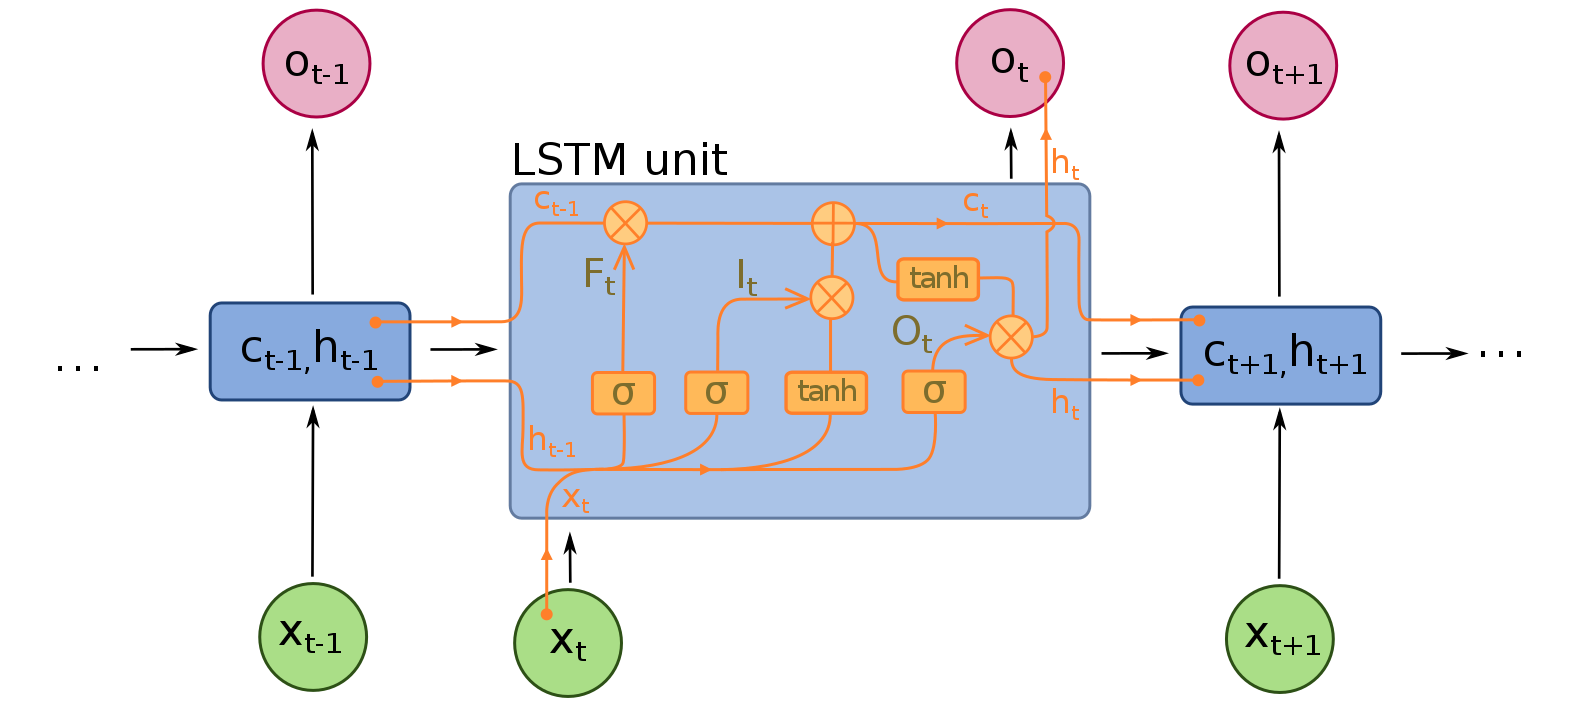
\includegraphics[width=12.5cm]{images/Long_Short-Term_Memory.png}
\end{figure}

Recurrent neural networks (RNNs) are a class of artificial neural network that use reasoning about previous events in the data to inform predictions \cite{olah}. In other words, RNNs retain state at one time to the next, using the previous state's output for the current estimate. This characteristic enables multi-stepped time series forecasting. A particular architecture of RNNs known as Long Short-Term Memory (LSTM) allows the model to recognize and retain short-term patterns for long periods of time \cite{hochreiter}. This architecture is used best where data from an earlier state needs to be recalled at a later state. Examples of LSTM networks in industry include Google Voice \cite{beaufays} and state-of-the-art performance on Google Translate \cite{le}.

\section{Object-Oriented Abstraction}
The working LSTM model was created in a Jupyter Notebook. While serving as a minimum proof of concept, the model should not require that the end-user engage directly with code. Furthermore, the following criteria were set: 1) the lifecycle of the model from training, testing, to final predictions needed to be automated and callable with a simple applicaition programming interface (API); 2) the Jupyter Notebook code (which executes similarly to a script) needed to be organized into an object-oriented structure to store data within the object instance; 3) the model needed to be capable of loading datasets of arbitrary products. Criterion (2) is more a matter of preference and style to the author, as other programming paradigms could be considered. The rest of this section briefly discusses the process involved in restructuring the model code to meet the criteria.

\subsection{Decomposition}
The goal of decomposition is to break a complex system into parts that are easier to understand, program, and maintain. The process of decomposing the Jupyter Notebook code involved defining separate modules for loading datasets (\texttt{data.py}), feature engineering (\texttt{features.py}), training/testing/predicting (\texttt{core.py}), and accessing utilities (\texttt{utils.py}). Furthermore, the code was organized into functions, and eventually into methods (discussed below).

\subsection{Encapsulation}
After breaking the code into manageable chunks, I created a Python class wrapper to store internal state and to allow the end-user to specify runtime options. The entire model can be run by using the wrapper's simple API.

\section{Hyperparameter Optimization}
Hyperparameter optimization deals with the learning parameters of a model rather than weights for features. While I made a significant effort in this area, the optimization was only run on one machine. Increasing compute resources to perform a more extensive search may yield further interesting results.

\subsection{Cross-validation}
\label{cross_validation}
In time series problems, cross-validation is performed chronologically with splits at fixed time intervals. In my trials, I ran cross-validation with 2, 3, and 10 splits. I wanted to understand the change in our key metric, MAPE (mean absolute percent error), as the number of splits $S$ increases. According to the \texttt{scikit-learn} documenation, the training set $Tr$ for the $i$th split has a size

\begin{equation}
  \label{eq:3}
  Tr_{i} = \floor*{\frac{i \times N}{(S + 1)}} + N \bmod (S + 1)
\end{equation}

where $N$ is the number of samples, $S$ is the number of splits, and $\floor{expression}$ denotes the floor function. Meanwhile, the test set $Te$ has the size shown in equation \ref{eq:4}.

\begin{equation}
  \label{eq:4}
  Te_{i} = \floor*{\frac{N}{(S + 1)}}
\end{equation}

For time series splits with $S>1$, the sum of the first train/test set is strictly less than $N$ and the last train/test set is equal to $N$:

\begin{equation}
  \label{eq:5}
  Tr_{i} + Te_{i} < N \quad \forall i \in \{1, \dots, S-1\}
\end{equation}

\begin{equation}
  \label{eq:6}
  Tr_{S} + Te_{S} = N
\end{equation}

These equations describe the train/test split pairs. It is important to note that the chronological indexing of the data is preserved for both input data and additional "held-out" data. This splitting strategy helps validate the results of the exhaustive hyperparameter search that is described in the next section.
\subsection{Grid Search}
This search algorithm is simple. It exhaustively generates candidate learning parameters and selects the best candidate based on the scoring function (MAPE). The number of candidates $C$ is equal to all possible combinations of user-specified parameter values. For $n$ parameters, the number of candidates is equal to

\begin{equation}
  C = \prod_{i=1}^{n} x_i
\end{equation}

\noindent where $x_i$ is the number of values for the $i$th parameter. Each candidate is fit using the time series split strategy discussed in Section \ref{cross_validation} to help validate the candidate's score. As a result, the number of fits is equal to the number of candidates times the number of splits.

\begin{equation}
  \text{F} = C \times S
\end{equation}

\noindent For further discussion about alternative parameter seearch algorithms, see Section \ref{improving_hyperparameter_optimization_efficiency}.

\subsection{Results}
Many trials with cross-validation were run, producing standardized output containing the learning parameters, test loss, and error metrics. Example output of this process is shown in Figure~\ref{fig:Example_Output}. Even though they are refitting multiple times, cross-validated trials completed very fast. The system is not so robust, failing $1/3$rd of the time; typically 300\% of the host machine's CPU usage was exceeded during failures. Although few learning parameters were tested, the cross-validation results are very consistent. We are reasonably sure that our model will perform well with unseen data. As a note, choosing the hyperparameters with higher cross-validation errors will help prevent overfitting when forecasting \cite{ng}.

\begin{table}
  \begin{center}
    \captionof{table}{Cross-validation Trials} \label{tab:cv_trials}
    \begin{tabular}{ l c c c c c c c r }
      Trial & Product & Length & MAPE & Runtime & Candidates & Splits & Fits & Failure \\
      \hline
      1 & 1 & 16 w & 5.13\% & 4:26 & 8 & 3 & 24 & - \\
      2 & 1 & 16 w & 5.06\% & 8:24 & 8 & 3 & 24 & - \\
      3 & 1 & 16 w & - & - & 8 & 3 & 24 & \checkmark \\
      \hline
      4 & 2 & 16 w & 4.13\% & 1:59 & 8 & 3 & 24 & - \\
      5 & 2 & 16 w & 4.28\% & 2:17 & 8 & 3 & 24 & - \\
      6 & 2 & 16 w & - & - & 8 & 3 & 24 & \checkmark \\
      \hline
      7 & 3 & 16 w & 	5.08\% & 2:04 & 8 & 3 & 24 & - \\
      8 & 3 & 16 w & 	- & - & 8 & 3 & 24 & \checkmark \\
      9 & 3 & 16 w & 	4.82\% & 2:10 & 8 & 3 & 24 & - \\
    \end{tabular}
  \end{center}
\end{table}

\begin{figure}[h]
  \caption{Example of grid search output}
  \label{fig:Example_Output}
  \begin{center}
    \begin{tabular}{c}
      \begin{lstlisting}
        Parameters: {
          'batch_size': 150,
          'epochs': 200,
          'optimizer': 'adam',
          'units': 100
        }
        Test loss: [128.97596047141334, 128.97596047141334]
        Testing set RMSE: 24318.87
        Testing set MAPE: 5.79%
        Testing set sMAPE: 0.06%
      \end{lstlisting}
    \end{tabular}
  \end{center}
\end{figure}

\section{Systems Engineering}
The goal at the onset was to develop a minimal machine learning system to avoid the problem of technical debt \cite{sculley}. I worked to productionize our model by building a back-end that is capable of extracting and preparing data, training and validating the model, and producing forecasts. The back-end performs the business logic computation without end-user interaction. The back-end was written entirely in Python and its component parts are discussed in this section.

\subsection{Server Infrastructure}
All software written for this project was developed and tested on local machines. System specifications of the host machine producing the results in this report are shown in Figure~\ref{fig:System_Specs}. The system runs Python 3.6.4 and we've tested on local machines (macOS) and a Docker virtual host container running Ubuntu 16.04. A simple web server framework, Flask (\url{http://flask.pocoo.org/}), is employed to interact with the front-end (see in Section \ref{user_interface}). A basic API has been developed to enable asynchronous communication with the front-end client device.

\begin{figure}[h]
  \caption{Host machine system information}
  \centering
  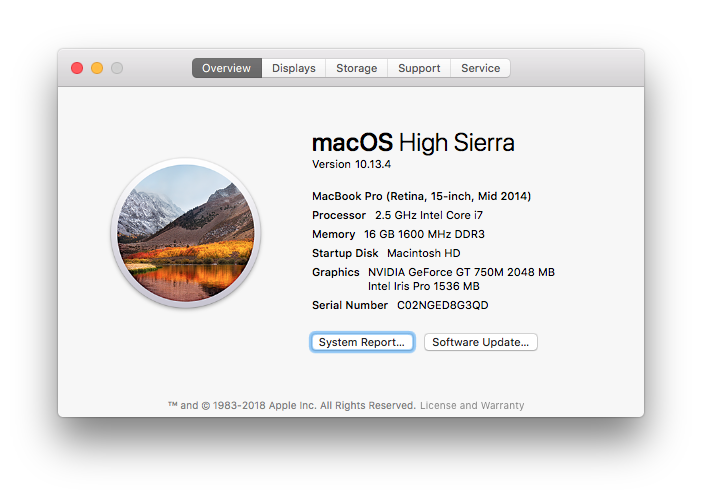
\includegraphics[width=12.5cm]{images/System_Specs.png}
  \label{fig:System_Specs}
\end{figure}

\subsection{Distributed Task Queue}
Since the machine learning processes are long-running processes, an open-source distributed task queue called Celery (\url{http://www.celeryproject.org/}) is used to manage scheduling, state changes, and output. When the user makes a new forecast, an API endpoint queues the task. In our case, there was only one client utilizing the queue at a time. However, the additional benefit of using a task queue is to coordinate background jobs. When the end-user begins a new forecast task, they receive a response from the server immediately. The code on the client polls another API endpoint every second to check the status of the forecast task. When the status appears successful, the server responds with the necessary data to render the visualizations on the client device, as well as summary statistics.

\section{User Interface}
\label{user_interface}
The user interface (UI) ties together my team's work on building an advanced machine-learning model and providing real value to Adobe senior management. Creating the UI was a careful process because it had to meet the needs of our industry sponsor (Adobe) and it had to integrate with our back-end. My general approach involved gathering requirements, sketching the UI, presenting the sketch for feedback, developing visual elements, and iterating.

\begin{figure}[h]
  \caption{Dashboard user interface}
  \centering
  \fbox{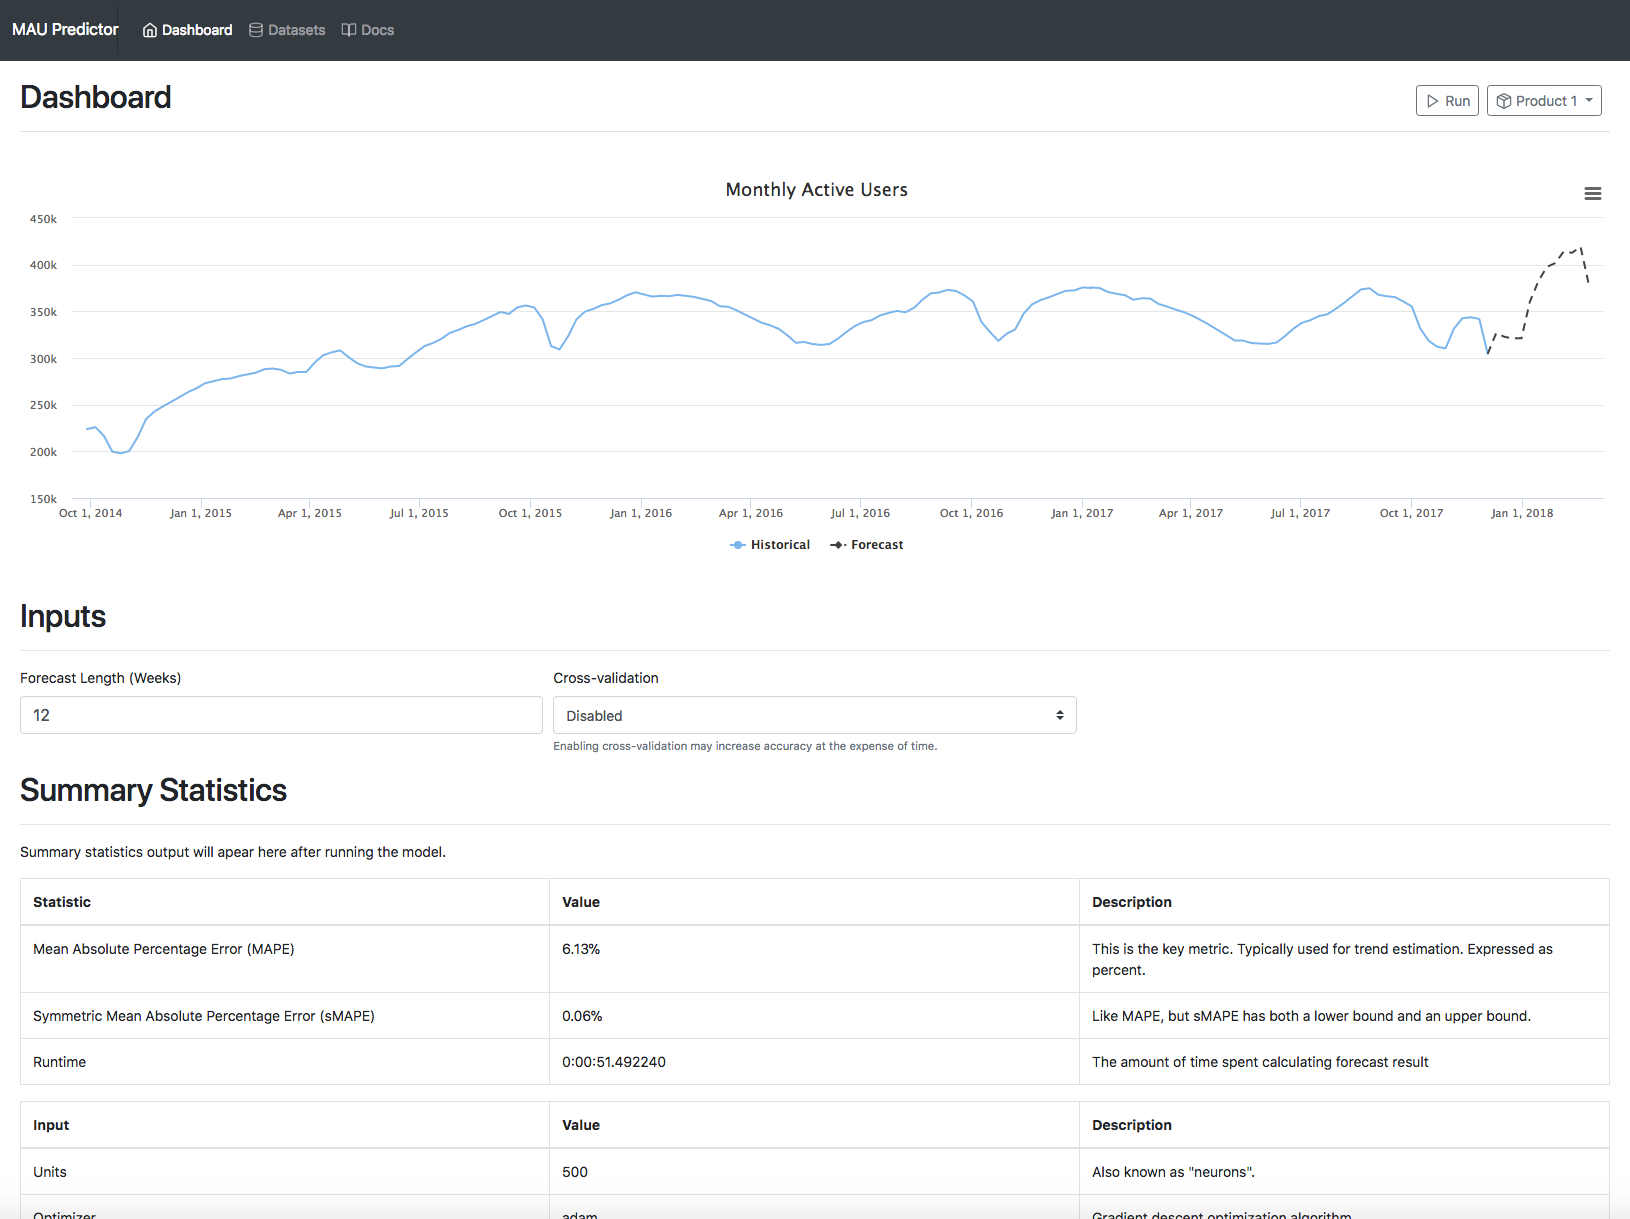
\includegraphics[width=12.5cm]{images/Dashboard.png}}
  \label{fig:Dashboard}
\end{figure}

\subsection{Forecast Visualization}
The forecast app shows a line chart of historical data and forecasted monthly active users. The end-user is able to isolate the forecast trendline and export the chart to various image formats. Charts related to forecasting are shown in the Appendix.

\subsection{Documentation}
I also wrote documentation for the forecasting app with three sections tailored to different stakeholder segments. The first section provides basic usage instructions for the non-technical end-user. The second section, tailored towards data scientists, goes more in-depth about the organization of the model code and how the cross-validation works. Lastly, the third section provides all technical documentation about the application itself, tailored towards developers.

\section{Next Steps}
\subsection{Websockets}
Currently, the forecast app polls the task status endpoint every second. The issue is that the task's status may not have changed, resulting in network overhead. Websockets provide a better alternative to HTTP. A websocket channel will enable the client device to subscribe to "events" from the back-end. For instance, when the task completes, the back-end can publish a new event that notifies the client device in real-time. However, websocket support with Flask may be limited and this improvement would not yield benefits unless the forecast app being used by multiple parties.

\subsection{Data Pipeline Automation (Apache Hive/Hadoop)}
Currently, new datasets must be moved to the project data folder manually. A future improvement may involve a direct connection to Adobe's Hive and Hadoop data services in order to automate the pull of new data. For instance, a SQL query editor may enable the end-user to create or modify new or previous queries to forecast on various datasets. Perhaps an intermediate step would involve an interface for managing CSV file datasets from within the host file system.

\subsection{Improving Hyperparameter Optimization Efficiency}
\label{improving_hyperparameter_optimization_efficiency}
The brute-force search algorithm used to optimize hyperparameters can probably be replaced with another. The \texttt{GridSearchCV} class from \texttt{scikit-learn} implements the algorithm that was used for our project, but other hyperparameter optimizers are available in the \texttt{model\_selection} module of \texttt{scikit-learn}. The other options include a randomized search where a subset of the parameter grid is sampled. This requires passing in distributions of the hyperparameters themselves, which could be an interesting opportunity to avoid an exhaustive search.

\section{Conclusion}
The forecast app creates 16 week forecasts in under 1 minute with a 5\% error rate and the results have been cross-validated. The model was productionized into a dashboard interface that can be deployed anywhere, for any product. There are still further steps that would improve the user experience and model accuracy. There is also further research to be conducted around verifying the efficacy of our model and for architectural improvements.

\chapter{Engineering Leadership}

\section{Project Management}
Project management was vital to the success of our engagement with Adobe. What helped our team is that one of our team members is an employee at Adobe who works in the field of project, program, and portfolio management. Hence, he has quite a bit of experience managing a large number of cross-functional and complex projects and programs and is certified as a ScrumMaster (CSM), certified as a Product Owner (CSPO) and has completed PMP training. Therefore, he was the driver and responsible for project managing this entire capstone engagement.

Generally, successfully managing a project comes down to whether or not a project can be delivered on time, within scope, and within budget without compromising on the quality. However, there is much more to that. It's very important to utilize effective channels of communication between all stakeholders. In our project, we used Slack during working hours to communicate within ourselves and to Adobe. However, during non-working hours, since Slack may not be checked in a timely manner and hence response times may increase, we decided to use WhatsApp as the primary form of instant communication. We established a weekly cadence of meeting remotely with Raghu Thricovil (Senior Manager of Creative Cloud Strategy and Analytics) and his team as they were our primary stakeholders from Adobe. We would discuss any open action items, as well as any risks, issues, blockers, and dependencies, and made sure these were all documented. The project plan, which was created by Nabeel, was used to determine if we were on track in terms of deliverables and deadlines. We'd leave each meeting with follow-up items that would need to be completed before the next weekly meeting and each item would have an owner assigned to it so that both parties (UC Berkeley and Adobe) knew who was in charge of that specific item.

There were several parts to this project and they all needed to be integrated together to have a working model ready for Adobe. Nabeel performed the Data Selection, Extraction, and Anonymization. All tasks were dependent on getting this data so this was high priority and a blocker for all other items. Once this was completed, Nabeel shared the data with the rest of the team and then performed descriptive analytics to get a sense of what the data was telling us. Farshad led the team in time series modeling and machine learning techniques and used a neural net for the model and this was not dependent on the work Nabeel was performing related to the descriptive analytics although the insights found were helpful. Hence, Farshad started on his tasks as soon as the data was shared. Matt focused on creating the GUI and this was dependent on Farshad's work since we had to incorporate the neural net frameworks into the GUI. Hence, we made sure to manage all these different workstreams and tracked dependencies.

\section{Technology Strategy}
Our technology was developed in partnership with Adobe, reserving them rights around intellectual property. The main idea at the onset was to use the technology internally to gather intelligence about monthly active (MAU) users across any product that had accumulated enough data. The use case had started to develop as progress in our project was made. Towards completion, we learned that Adobe has groups of teams for each product with their own product managers who can get value from the forecasting dashboard. Thus, the technology can be deployed internally to these teams. The historical data and forecast visualizations are new tools, and can enable the product managers, data scientists, and non-technical employees to monitor and analyze usage trends and to detect anomalies in the data.

Initially, we will prosthelytize the Data Practitioners Group (DPG) within Adobe to demonstrate the value of the forecasting dashboard and to encourage them to use it. Various product managers, data scientists, engineers, and researchers will learn about the technology's capabilities so we can spread adoption within the organization. It is important that experts in data analytics as well as non-technical product teams adopt the solution together. This way, if any technical difficulties arise around installation, bugs, or system failures, then the problems can be jointly tackled. We realize that there is still room for upgrades to our technology and system and in order to meet unscoped yet pressing needs within the company, additional features may be added.

After the internal deployment, further use cases may arise; other functional teams, such as finance and accounting, may find the tool useful for forecasting product revenues. In software-as-a-service companies, monthly active usage data helps inform rates of growth in free vs. paid adoption. It is possible to segment the monthly active usage data between free and paid users, allowing the finance department to forecast growth in revenue. Forecasting revenue may require a separate model, but it can be as simple as a regression model where revenue is regressed on paid monthly active users. After determining the regression coefficient, the paid monthly active users forecast can be the input to forecast revenue. Such a model doesn't require anything fancy; financial operations analysts should be able to perform the regression in an Excel spreadsheet.

A revenue forecast can be a very powerful indicator. Adobe may choose to provide financial analysts from Wall Street guidance based on forecasted revenue produced from our technology during quarterly earnings calls. This would help the investor community and Adobe to maintain a fair stock price. Should the technology evolve to this level, the strategy might change. While such a technology could be commercialized and of use to the public domain, the application of the technology does not fit any Adobe product line. Depending on the public need at the time, the technology may have open-source adoption potential.

\section{Data Analytics}
Understanding the data provided by Adobe and uncovering hidden patterns in user behaviors as it pertains to MAU is critical to the model development. Data analytics, and more broadly machine learning, is analogous to the engine of a car.  No matter how pretty or affordable the car is, if the engine does not run properly or efficiently, then one can argue that the car is useless.  Just as it's critical to build the right engine for the right car, it's critical to build the right model to solve the appropriate business problem.

George Box, a famous statistician, claims that "all models are wrong; some are useful" (Box, 2005). That being said, it is important to evaluate the tradeoffs between models given the business context. Adobe sees business value, such as forecasting revenue growth by predicting MAU for their Creative Cloud products. Furthermore, as mentioned earlier, Adobe managers understand the inherent uncertainty in all models and thus want the benefits of toggling various levers (or inputs) in order to observe the impacts to the output. This interactivity enables senior management to sit in a room and dynamically challenge each other's inputs and perform real-time sensitivity analysis on the model.
Two major considerations had to be made in building a model to handle time series data. The first approach entails using a traditional ARIMA model where autocorrelations, seasonality, and trends can quickly be fitted to produce a reasonable forecast. An ARIMA model is made available out-of-the-box by an open-source software tool developed by Facebook called Prophet (Taylor, 2017).  During model exploration, this tool allowed for quick solutions, interpretable models, and fairly simple accounting for "holidays" or in the case of Adobe products, "feature releases".  In contrast however, the alternative was to implement a recurrent neural network model that has a much higher forecasting accuracy but can potentially be slower and less interpretable for management.

Through further strategic discussions with Adobe, the path chosen for purposes of this project was to develop a neural network with an objective to forecast MAU as accurately as possible. However, the GUI built on top of the model can help alleviate the interpretability challenge and make the model appear less as a black-box and more as an instrument that management can interact with directly. With that said, Facebook's open source tool still remains a viable and promising technology that the Adobe team can leverage for quick, out-of-the-box solutions.

Although performing data analytics and developing machine learning algorithms relies heavily on the hard skills (e.g., math and computer science), the huge, and often underappreciated opportunity resides in the soft skills. Being able to effectively communicate what may appear as a black-box to all stakeholders, whether they are fellow engineers, management, or even lawyers, can be of much more value than a model with improved accuracy. That communication entails education around model selection, its relevance to the business context, and ultimately, working with the Adobe engineering team to educate them on the model mechanics and dependencies---which will be critical for integrating it into their daily operations.

\newpage
\bibliographystyle{apacite}
\bibliography{references}

\newpage
\begin{appendices}
  \begin{figure}[h]
    \caption{Product 1 trend: 6.24\% MAPE}
    \centering
    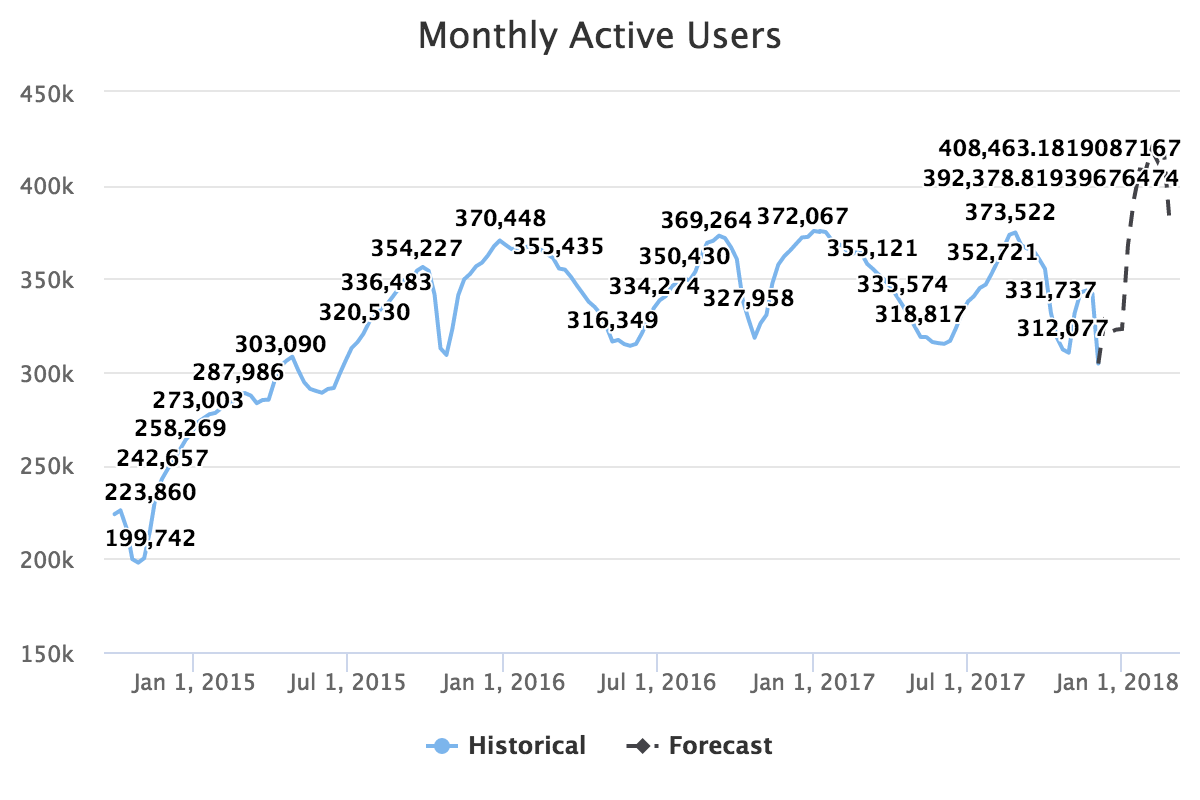
\includegraphics[width=12.5cm]{images/Product_1-Trend-6_24_Percent_MAPE.png}
    \label{fig:Product_1-Trend}
  \end{figure}

  \begin{figure}[h]
    \caption{Product 1 forecast: 6.24\% MAPE}
    \centering
    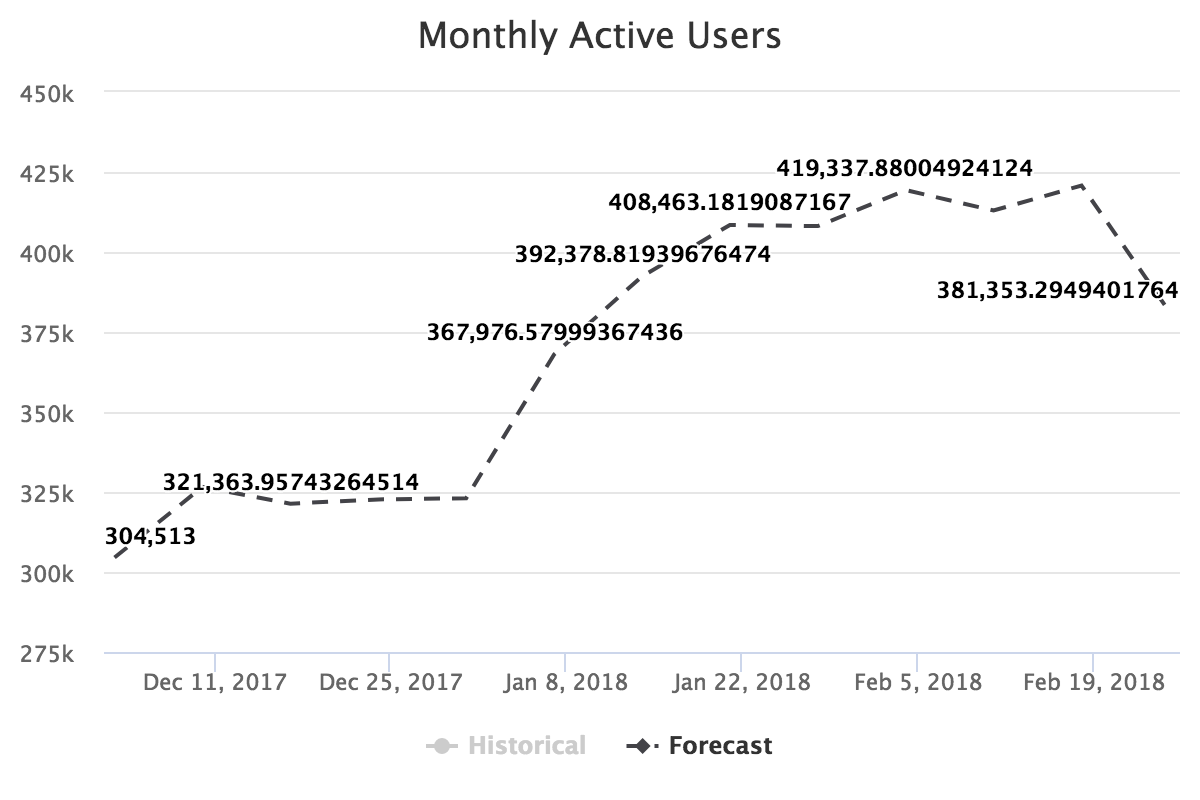
\includegraphics[width=12.5cm]{images/Product_1-Forecast-6_24_Percent_MAPE.png}
    \label{fig:Product_1-Forecast}
  \end{figure}

  \begin{figure}[h]
    \caption{Product 2 trend: 6.05\% MAPE}
    \centering
    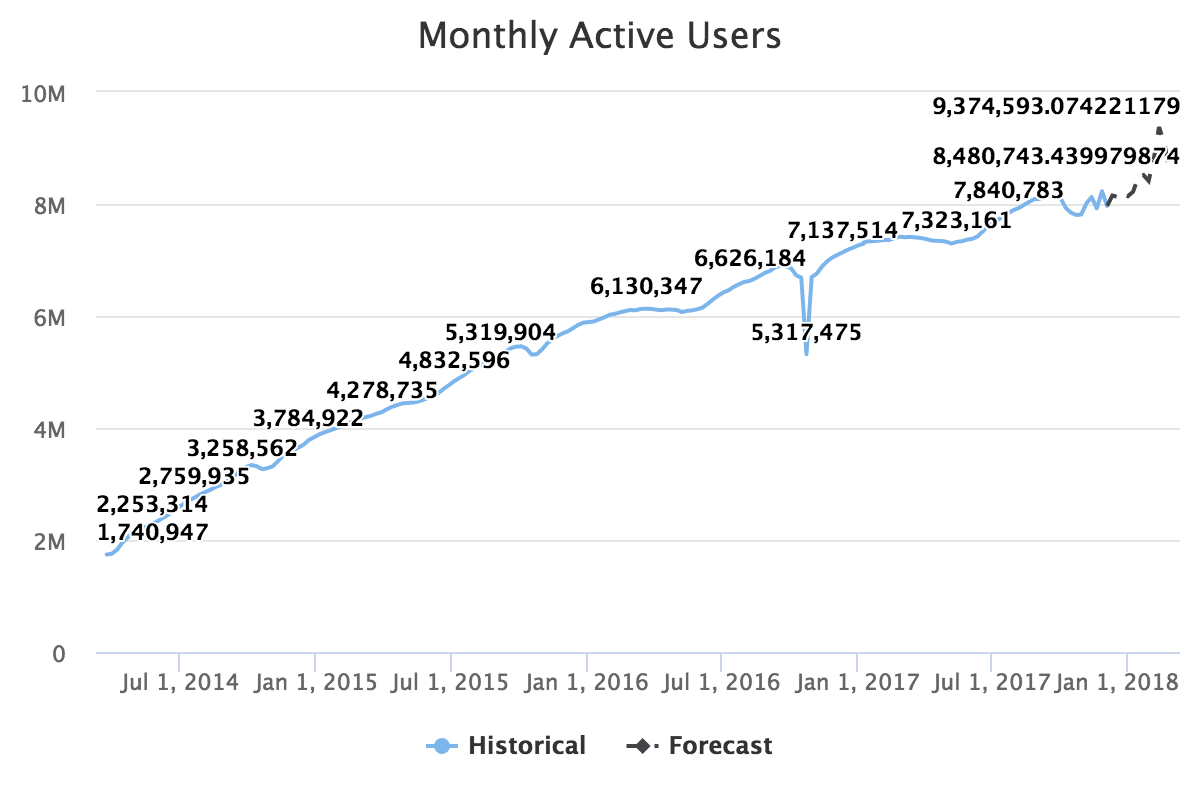
\includegraphics[width=12.5cm]{images/Product_2-Trend-6_05_Percent_MAPE.png}
    \label{fig:Product_2-Trend}
  \end{figure}

  \begin{figure}[h]
    \caption{Product 2 forecast: 6.05\% MAPE}
    \centering
    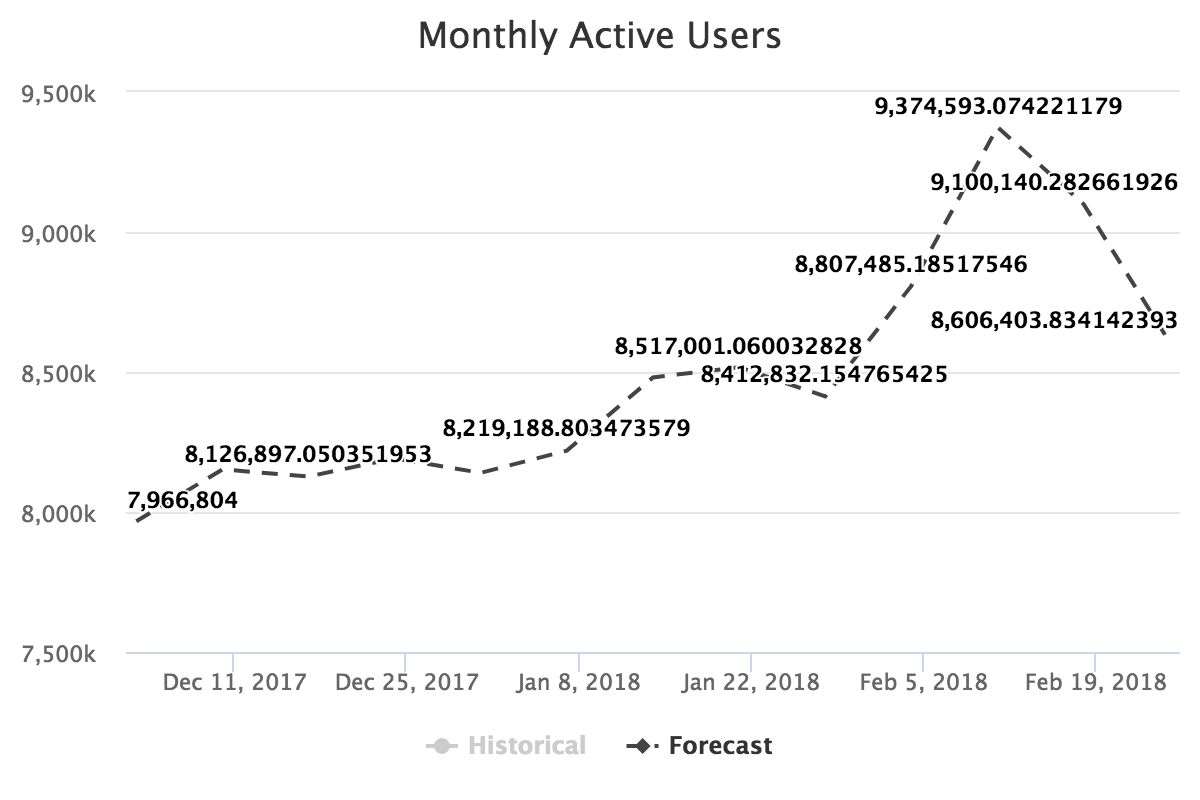
\includegraphics[width=12.5cm]{images/Product_2-Forecast-6_05_Percent_MAPE.png}
    \label{fig:Product_2-Forecast}
  \end{figure}

  \begin{figure}[h]
    \caption{Product 3 trend: 4.82\% MAPE}
    \centering
    \includegraphics[width=12.5cm]{images/Product_3-Trend-4_82_Percent_MAPE.png}
    \label{fig:Product_3-Trend}
  \end{figure}

  \begin{figure}[h]
    \caption{Product 3 forecast: 4.82\% MAPE}
    \centering
    \includegraphics[width=12.5cm]{images/Product_3-Forecast-4_82_Percent_MAPE.png}
    \label{fig:Product_3-Forecast}
  \end{figure}
\end{appendices}

\end{document}
